%!TEX root = ../OGUSAdoc.tex

In this chapter, we define the stationary steady-state equilibrium of the \ogindia model. Chapters \ref{Chap_Demog} through \ref{Chap_MarkClr} derive the equations that characterize the equilibrium of the model. However, we cannot solve for any equilibrium of the model in the presence of nonstationarity in the variables. Nonstationarity in \ogindia comes from productivity growth $g_y$ in the production function \eqref{EqFirmsCESprodfun}, population growth $\tilde{g}_{n,t}$ as described in Chapter \ref{Chap_Demog}, and the potential for unbounded growth in government debt as described in Chapter \ref{Chap_UnbalGBC}.

We implemented an automatic government budget closure rule using government spending $G_t$ as the instrument that stabilizes the debt-to-GDP ratio at a long-term rate in \eqref{EqUnbalGBCclosure}. And we showed in Chapter \ref{Chap_Stnrz} how to stationarize all the other characterizing equations.


\section{Stationary Steady-State Equilibrium Definition}\label{SecEqlbSSdef}

  With the stationarized model, we can now define the stationary steady-state equilibrium. This equilibrium will be long-run values of the endogenous variables that are constant over time. In a perfect foresight model, the steady-state equilibrium is the state of the economy at which the model settles after a finite amount of time, regardless of the initial condition of the model. Once the model arrives at the steady-state, it stays there indefinitely unless it receives some type of shock or stimulus.

  These stationary values have all the growth components from productivity growth and population growth removed as defined in Table \ref{TabStnrzStatVars}. Because the productivity growth rate $g_y$ and population growth rate series $\tilde{g}_{n,t}$ are exogenous. We can transform the stationary equilibrium values of the variables back to their nonstationary values by reversing the identities in Table \ref{TabStnrzStatVars}.

  \vspace{5mm}
  \hrule
  \vspace{-1mm}
  \begin{definition}[\textbf{Stationary steady-state equilibrium}]\label{DefSSEql}
    A non-autarkic stationary steady-state equilibrium in the \ogindia model is defined as constant allocations of stationary household labor supply $n_{j,s,t}=\bar{n}_{j,s}$ and savings $\hat{b}_{j,s+1,t+1}=\bar{b}_{j,s+1}$ for all $j$, $t$, and $E+1\leq s\leq E+S$, and constant prices $\hat{w}_t=\bar{w}$ and $r_t=\bar{r}$ for all $t$ such that the following conditions hold:
    \begin{enumerate}
      \item the population has reached its stationary steady-state distribution $\hat{\omega}_{s,t} = \bar{\omega}_s$ for all $s$ and $t$ as characterized in Section \ref{SecDemogPopSSTP},
      \item households optimize according to \eqref{EqStnrzHHeul_n}, \eqref{EqStnrzHHeul_b}, and \eqref{EqStnrzHHeul_b},
      \item firms optimize according to \eqref{EqStnrzFOC_L} and \eqref{EqFirmFOC_K},
      \item Government activity behaves according to \eqref{EqStnrzGovBC} and \eqref{EqStnrzClosureRule}, and
      \item markets clear according to \eqref{EqStnrzMarkClrLab}, \eqref{EqStnrzMarkClrCap}, and \eqref{EqStnrzMarkClrBQ}.
    \end{enumerate}
  \end{definition}
  \vspace{-2mm}
  \hrule
  \vspace{5mm}


\section{Stationary Steady-state Solution Method}\label{SecEqlbSSsoln}

  \renewcommand\theenumi{\arabic{enumi}}
  \renewcommand\theenumii{\alph{enumii}}
  \renewcommand\theenumiii{\roman{enumiii}}

  This section describes the solution method for the stationary steady-state equilibrium described in Definition \ref{DefSSEql}. The steady-state is characterized by $2JS$ equations and $2JS$ unknowns. However, because some of the other equations cannot be solved for analytically and substituted into the Euler equations, we use a fixed point algorithm to solve for the steady-state. We begin by making a guess at steady-state interest rate $\bar{r}$, total bequests $\overline{BQ}$, total household transfers $\overline{TR}$, and income multiplier $factor$. We call these four steady-state variables the ``outer loop'' variables in our steady-state solution method and the determination of a fixed point over these variables the ``outer loop'' of the steady-state solution method. The outer loop variables are the macroeconomic variables necessary to solve the household's problem.

  For each iteration over these outer-loop variables, we solve the household problem given the values of these macroeconomic variables.  We call this solution the ``inner loop'' of the steady-state solution method.  In the inner loop, we solve for the steady-state household decisions $\bar{b}_{j,s}$ and labor supply $\bar{n}_{j,s}$ for all $j$ and $E+1\leq s\leq E+S$, and then use the household decisions to compute updated values for macroeconomics variables. Because the lifetime optimization problem of each household of type $j$ is a highly nonlinear system of $2S$ equations and $2S$ unknowns, we solve for the $2S$ household's decisions simultaneously for a given type $j$ household.  We then use the solutions for type-$j$ households as the initial guesses a the solutions for type-$j+1$ households.

  The macroeconomic variables computed from the solutions to the household problem are used to update the values of those macroeconomic variables in the outer-loop.  This process continues until a fixed point is found.  That is, until the macroeconomic variables in the outer loop result in household decisions that are consistent with those macroeconomic variables' values.

 We outline this algorithm in the following steps.

  \begin{enumerate}
    \item Use the techniques from Section \ref{SecDemogPopSSTP} to solve for the steady-state population distribution vector $\bm{\bar{\omega}}$ and steady-state growth rate $\bar{g}_n$ of the exogenous population process.
    \item Choose an initial guess for the values of the steady-state interest rate $\bar{r}^i$, total bequests $\overline{BQ}^{\,i}$, total household transfers $\overline{TR}^{\,i}$, and income multiplier $factor^i$, where superscript $i$ is the index of the iteration number of the guess.
    \item Use $\bar{r}^i$ together with the firm's first order condition for its choice of capital, Equation \ref{EqFirmFOC_K}, to solve for the capital labor ratio, $\frac{\overline{K}}{\overline{L}}$.  Then use $\frac{\bar{K}}{\bar{L}}$ in the firm's first order condition for its choice of labor to find the implied wage rate $\bar{w}^i$.
    \item Given guesses for $\bar{r}^i$, $\bar{w}^i$, $\overline{BQ}^{\,i}$, $\overline{TR}^{\,i}$, and $factor^i$, solve for the steady-state household labor supply $\bar{n}_{j,s}$ and savings $\bar{b}_{j,s}$ decisions for all $j$ and $E+1\leq s\leq E+S$.
    \begin{enumerate}
      \item Do this by using a multivariate root-finder to solve the $2S$ necessary conditions of the household given by Equations \ref{EqHHeul_n}, \eqref{EqHHeul_b}, and \eqref{EqHHeul_bS} simultaneously for $j=1$.
      \item Repeat this root-finding process for each household $j\in{2,...,J}$, using the solutions for households of type $j-1$ as the initial guesses in the root-finder.
   \end{enumerate}
    \item Given partial equilibrium household steady-state solutions $\{\bar{c}_{j,s},\bar{n}_{j,s},\bar{b}_{j,s+1}\}_{s=E+1}^{E+S}$ based on macroeconomic variables $\bar{r}^i$, $\overline{BQ}^{\,i}$, $\overline{TR}^{\,i}$, and $factor^i$, compute updated values for the outer loop macroeconomic variables, $\bar{r}^{i'}$, $\bar{w}^{i'}$, $\overline{BQ}^{\,i'}$, $\overline{TR}^{\,i'}$, and $factor^{i'}$ .
    \begin{enumerate}
      \item We solve for the updated interest rate as follows:
      	\begin{enumerate}
      		\item Use the guess at total transfers, $\overline{TR}^{i}$ and the transfer spending rule given in Equation \eqref{EqUnbalGBCtfer} to find the implied GDP: $\bar{Y}^{i} = \frac{\overline{TR}^{i}}{\alpha_{tr}}$.
      		\item Use the long-run debt-to-GDP ratio and $\bar{Y}^{i}$ to find total government debt in the steady-state, $\bar{D}^{i} = \alpha_{D}\bar{Y}^{i}$.
      		\item Use the capital market clearing condition from Equation \eqref{EqStnrzMarkClrCap} and $\bar{D}^{i}$ to find aggregate capital,

      		\begin{equation*}
      			\bar{K}^{i}=\frac{1}{1 + \bar{g}_{n}}\sum_{s=E+2}^{E+S+1}\sum_{j=1}^{J}\Bigl(\bar{\omega}_{s-1}\lambda_j \bar{b}_{j,s} + i_s\bar{\omega}_{s}\lambda_j \bar{b}_{j,s}\Bigr) - \bar{D}^{i}
      		\end{equation*}

      		\item Use the labor market clearing condition from Equation \eqref{EqStnrzMarkClrLab} to find aggregate labor supply:

      		\begin{equation*}
      			\bar{L}^{i}=\sum_{s=E+1}^{E+S}\sum_{j=1}^{J} \bar{\omega}_{s}\lambda_j e_{j,s}\bar{n}_{j,s}
      		\end{equation*}

      		\item Use the firm's production function from Equation \eqref{EqStnrzCESprodfun} to compute an updated value of $\bar{Y}$ given the values for the factors of production:

      		\begin{equation*}
      			\bar{Y}^{i'} = \bar{Z}\biggl[(\gamma)^\frac{1}{\ve}(\bar{K}^{i})^\frac{\ve-1}{\ve} + (1-\gamma)^\frac{1}{\ve}(\bar{L}^{i})^\frac{\ve-1}{\ve}\biggr]^\frac{\ve}{\ve-1}
      		\end{equation*}

      		\item Use the firm's first order condition for its choice of capital to find the updated interest rate,

      		\begin{equation*}
      		\bar{r}^{i'} = (1 - \tau^{corp})(\bar{Z})^\frac{\ve-1}{\ve}\left[\gamma\frac{\bar{Y}^{i'}}{\bar{K}^{i}}\right]^\frac{1}{\ve} - \delta + \tau^{corp}\delta^\tau
      		\end{equation*}

      		\end{enumerate}
      by first using the market clearing conditions \eqref{EqStnrzMarkClrLab} and \eqref{EqStnrzMarkClrCap} together with the the long-run debt


      \item The stationarized law of motion for total bequests \eqref{EqStnrzMarkClrBQ} provides the expression in which household savings decisions $\{\bar{b}_{j,s+1}\}_{s=E+1}^{E+S}$ imply a value for aggregate bequests, $\overline{BQ}^{\,i'}$. When computing aggregate bequests, we use the updated interest rate found above.
      \begin{equation*}
        \overline{BQ}^{\,i'} = \left(\frac{1+\bar{r}^{i'}}{1 + \bar{g}_{n}}\right)\left(\sum_{s=E+2}^{E+S+1}\sum_{j=1}^J\rho_{s-1}\lambda_j\bar{\omega}_{s-1}\bar{b}_{j,s}\right)
      \end{equation*}

      \item In equation \eqref{EqStnrzTfer}, we defined total household transfers as a fixed percentage of GDP ($\overline{TR}=\alpha_{tr}\bar{Y}$).  To find the updated value for transfers, we find the amount of transfers implied by the most updated value of GDP, $\overline{TR}^{i'}=\alpha_{tr}\bar{Y}^{i'}$.




      \item The $factor$ that transforms the model units to U.S. dollar units for the tax functions \eqref{EqTaxCalcFactor} is already defined in terms of steady-state variables. The following is an expression in which household decisions $\{\bar{n}_{j,s},\bar{b}_{j,s+1}\}_{s=E+1}^{E+S}$ imply a value for the steady-state $factor^{i'}$. Note, as with the equation for $\overline{BQ}^{\,i'}$, that we include the updated values of $\bar{w}^{i'}$ and $\bar{r}^{i'}$ on the right-hand-side of the equation.\footnote{The updated wage rate, $w^{i'}$, is found by using the updated interest rate, $r^{i'}$ as detailed in Step 3.}
      \begin{equation*}
        factor^{i'} = \frac{\text{Avg. household income in data}}{\sum_{s=E+1}^{E+S}\sum_{j=1}^J\lambda_j\bar{\omega}_s\left(\bar{w}^{i'}e_{j,s}\bar{n}_{j,s} + \bar{r}^{i'}\bar{b}_{j,s}\right)}
      \end{equation*}

      \end{enumerate}
  \item The updated values for the outer loop variables are then used to compute the percentage differences between the initial and implied values:
  	\begin{enumerate}
  		\item $error_r = \frac{\bar{r}^{i'} - \bar{r}^i}{\bar{r}^i}$
  		\item $error_{bq} = \frac{\overline{BQ}^{\,i'} - \overline{BQ}^{\,i}}{\overline{BQ}^{\,i}}$
  		\item $error_{tr} = \frac{\overline{TR}^{\,i'} - \overline{TR}^{\,i}}{\overline{TR}^{\,i}}$
  		\item $error_f = \frac{factor^{i'} - factor^i}{factor^i}$
  	\end{enumerate}
   \item If the maximum absolute error among the four outer loop error terms is greater than some small positive tolerance $toler_{ss,out}$,
    \begin{equation*}
      \max\big|\left(error_r,error_{bq},error_{tr},error_f\right)\bigr| > toler_{ss,out}
    \end{equation*}
    then update the guesses for the outer loop variables as a convex combination governed by $\xi_{ss}\in(0,1]$ of the respective initial guesses and the new implied values and repeat steps (3) through (5).\footnote{In our code, there is also an option to use a Newton based root-finding algorithm to updated the outer-loop variables.  Such an algorithm is generally faster, but less robust than the functional iteration method outlined here.}
    \begin{equation*}
      \begin{split}
        \left[\bar{r}^{i+1},\overline{BQ}^{\,i+1},\overline{TR}^{\,i+1},factor^{i+1}\right] &= \xi_{ss}\left[\bar{r}^{i'},\overline{BQ}^{\,i'},\overline{TR}^{\,i'},factor^{i'}\right] + \\
        &\qquad(1-\xi_{ss})\left[\bar{r}^{i},\overline{BQ}^{\,i},\overline{TR}^{\,i},factor^{i}\right]
      \end{split}
    \end{equation*}
    \item If the maximum absolute error among the four outer loop error terms is less-than-or-equal-to some small positive tolerance $toler_{ss,out}$,
    \begin{equation*}
      \max\big|\left(error_r,error_{bq},error_{tr},error_f\right)\bigr| \leq toler_{ss,out}
    \end{equation*}
    then the steady-state has been found.
    \begin{enumerate}
      \item Make sure that steady-state government spending is nonnegative $\bar{G}\geq 0$. If steady-state government spending is negative, that means the government is getting resources to supply the debt from outside the economy each period to stabilize the debt-to-GDP ratio. $\bar{G}<0$ is a good indicator of unsustainable policies.
      \item Make sure that the resource constraint (goods market clearing) \eqref{EqStnrzMarkClrGoods} is satisfied. It is redundant, but this is a good check as to whether everything worked correctly.
      \item Make sure that the government budget constraint \eqref{EqStnrzGovBC} binds.
      \item Make sure that all the $2JS$ household Euler equations are solved to a satisfactory tolerance.
    \end{enumerate}
  \end{enumerate}

  \renewcommand\theenumi{\roman{enumi}}


\section{Baseline Steady-state Results}\label{SecSSeqlbResults}

  In this section, we use the baseline calibration described in Chapter \ref{Chap_Calibr}, which includes the baseline tax law from \taxcalc, to show some steady-state results from \ogindia. Figure \ref{FigSSeqlbHHvars} shows the household steady-state variables by age $s$ and lifetime income group $j$.

  \begin{figure}[htb]\centering \captionsetup{width=6.0in}
    \caption{\label{FigSSeqlbHHvars}\textbf{Steady-state distributions of household consumption $\bar{c}_{j,s}$, labor supply $\bar{n}_{j,s}$, and savings $\bar{b}_{j,s+1}$}}
    \begin{subfigure}[b]{0.48\textwidth}
      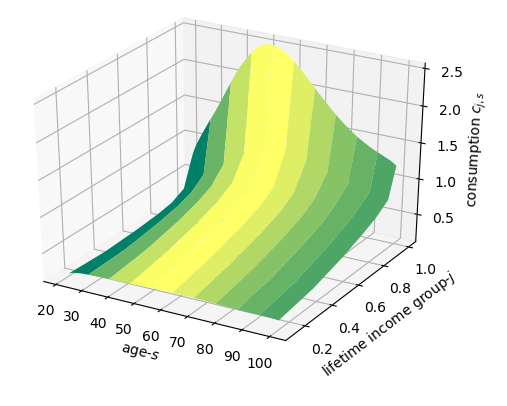
\includegraphics[width=\textwidth]{images/HHcons_SS.png}
      \caption{Consumption $\bar{c}_{j,s}$}
      \label{FigSSeqlbHHcons}
    \end{subfigure}
    \begin{subfigure}[b]{0.48\textwidth}
      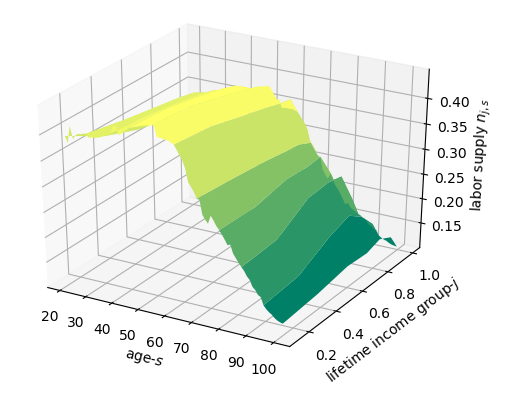
\includegraphics[width=\textwidth]{images/HHlab_SS.png}
      \caption{Labor supply $\bar{n}_{j,s}$}
      \label{FigSSeqlbHHlab}
    \end{subfigure}
    \begin{subfigure}[b]{0.48\textwidth}
      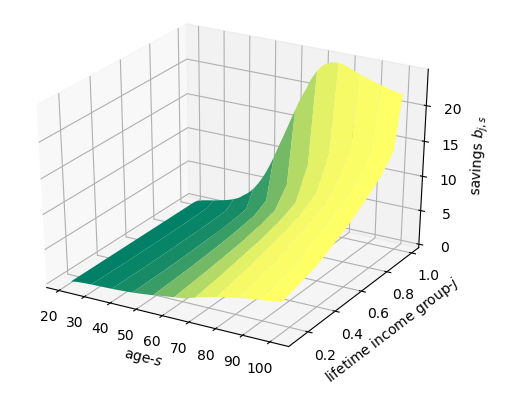
\includegraphics[width=\textwidth]{images/HHsav_SS.png}
      \caption{Savings $\bar{b}_{j,s+1}$}
      \label{FigSSeqlbHHsav}
    \end{subfigure}
  \end{figure}

  Table \ref{TabSSeqlbAggrVars} lists the steady-state prices and aggregate variable values along with some of the maximum error values from the characterizing equations.

  \begin{table}[htbp] \centering \captionsetup{width=4.1in}
  \caption{\label{TabSSeqlbAggrVars}\textbf{Steady-state prices, aggregate variables, and maximum errors}}
    \begin{threeparttable}
    \begin{tabular}{>{\small}l >{\small}r |>{\small}l >{\small}r}
      \hline\hline
      \multicolumn{1}{c}{\small{Variable}} & \multicolumn{1}{c}{\small{Value}} & \multicolumn{1}{c}{\small{Variable}} & \multicolumn{1}{c}{Value} \\
      \hline
      $\bar{r}$ & 0.058 & $\bar{w}$ & 1.148 \\
      \hline
      $\bar{Y}$ & 0.630 & $\bar{C}$ & 0.462 \\
      $\bar{I}$ & 0.144 & $\bar{K}$ & 1.810 \\
      $\bar{L}$ & 0.357 & $\bar{B}$ & 2.440 \\
      $\overline{BQ}$ & 0.106 & $factor$  & 141,580 \\
      \hline
      $\overline{Rev}$ & 0.096 & $\overline{TR}$ & 0.057 \\
      $\bar{G}$ & 0.023 & $\bar{D}$ & 0.630 \\
      \hline
      Max. abs.         & 4.57e-13 & Max. abs.  & 8.52e-13 \\[-2mm]
      \:\: labor supply &   & \:\: savings &     \\[-2mm]
      \:\: Euler error  &   & \:\: Euler error & \\
      Resource        & -4.39e-15 & Serial & 1 hr. 25.9 sec.\tnote{*} \\[-2mm]
      \:\: constraint & & \:\: computation & \\[-2mm]
      \:\: error      & & \:\: time &  \\
      \hline\hline
    \end{tabular}
    \begin{tablenotes}
      \scriptsize{\item[*]The steady-state computation time does not include any of the exogenous parameter computation processes, the longest of which is the estimation of the baseline tax functions which computation takes 1 hour and 15 minutes.}
    \end{tablenotes}
    \end{threeparttable}
  \end{table}
